\chapter{TRADITIONAL METHODS}\label{traditional_methods}

There are many different methods used for image inpainting. Each of these methods has mathematical foundations in itself. The first of these methods are the methods called traditional methods that try to correct the missing part on the main title picture only with the features in the picture to be corrected.

Machine learning methods, which have been used frequently in many different problems due to increased processing power and broad access to large data sets, have also started to be used for image inpainting problems. These ideas, which will be explained under the title of traditional methods, also formed the basis for machine learning and deep learning methods used for inpainting. The methods explained under this title were used in different deep learning methods, which will be examined later.

It would be more accurate to examine traditional methods mainly as exemplar-based and diffusion based. Although Exemplar-based methods are divided into pixel-based and patch-based, patch-based methods will be examined mainly in exemplar-based methods, since there are more studies relating to patch-based methods and they give better results.

As can be understood from their names, patch-based methods try to fill the missing region in the picture with the information obtained from different parts of the picture. [References to different papers can be found here.]. Diffusion-based methods [1 2 sentence definition by Enes]

Traditional methods are methods that do not require training. For this reason, it is an appropriate method to use for simpler problems. Traditional methods do not work well in problems where the masked area in the picture starts to form a proportionally large area. This result is quite normal given that these methods infer from pixels near the missing region.

\section{Patch-based Methods}

Patch-based image inpainting consists of methods that use the undamaged regions in the image to create the region to be filled. With this approach it is aimed to have the highest possible patch similarity level.

In order to implement this method, an algorithm is needed on how to transfer the obtained regions to the areas planned to be filled. Another important point in this method is the selection of the algorithm that will compare the regions in different parts of the picture with the regions desired to be created [PatchMatch Ref].

While patch-based methods work well, they assume that the information in the missing part of the picture resides elsewhere in the picture. Another problem with patch-based methods is that they require relatively more processing power because they are methods that consistently involve searching and comparing.

\subsection{Patch-based Texture Synthesis}

In this method by Zhou et al [Ref], it is aimed to fill the desired area by creating textures with patch-based algorithms for Image inpainting method. While implementing this targeted method, a road starting from the rough, proceeding in detail is aimed. While performing the filling process, targets and constraints were created in order to ensure the integrity of the newly created region with the rest of the picture.

In this study, a more efficient inpainting study has been achieved by basically using the successive elimination algorithm and based on the previously used methods.

Texture synthesis is performed by trying to imitate information about texture and structure integrity. At the same time, it is aimed to reduce the processing power used by using the successive elimination algorithm during texture comparison.

In this approach, the function given in equation [] is tried to be minimized in order to achieve the desired result.

\begin{equation}
    buraya equation gelecek
\end{equation}

However, minimizing this equation does not mean that the energy function decreases in general. To explain better, the region to be filled in the image can be completely filled with a smaller patch than itself and gives a perfect result in the equation. However, for better results, coarse images as  are used in equation [] and equation [].

\begin{equation}
    buraya equation gelecek
\end{equation}

In this way, the image inpainting process for the visual is corrected to give a good result from the rough approach. However, this process requires a high processing power due to 3 different partial differential equations.

It is logical to use an approach to solve this problem. With this approach, uniform visual densities can be accepted as constant for different regions. Hence, MS energy function can be reduced to equation []. Also, an inpainted image example with its input image is given in figure [].

\begin{equation}
    buraya equation gelecek
\end{equation}

\begin{figure}[h]
    \centering
    \includegraphics{}
    \caption{Inpainted Image with Patch Based Texture Synthesis}
    \label{fig:my_label}
\end{figure}

\subsection{Image Melding}

The image melting method [Ref] creates a transition zone to transfer various information and properties within one image to another image. This method can be used for different purposes depending on the usage type.

This method, primarily uses many different transforms to increase the ability to search for patches. Next, image gradients are included in patch representation and Poisson equation solver is used for color averaging. Without causing blurry areas in the picture, a new energy method is used based on L2/L0 norms for colors. Melding of 2 different image is illustrated below in figure [].

\begin{figure}[h]
    \centering
    \includegraphics{}
    \caption{Image Melding Example}
    \label{fig:my_label}
\end{figure}

Many different patch-based methods have been used for inpainting problems. Image melding is basically a patch-based algorithm. However, when based-patched methods are given inconsistent visuals, they can give insufficient results because they use a direct distance function between pixels.

Another result aimed with this study is that patch-based and gradient methods can be used together and thus more complex problems can be solved. Thanks to the methods used, Image Melding can be used to solve many different problems including inpainting.

Image synthesis using a single source is one of the ways image melding can be used. In this algorithm, a mask divides the image into two parts, S and T, respectively, as source and target. After this process, the energy function shown in equation [] is obtained.

\begin{equation}
    buraya equation gelecek
\end{equation}

In the above equation Q represents the targeted patch with w width and height and target pixel q on the upper left corner. P represents the transformation that is applied to the neighbor pixels of the source pixel. Throughout the operations, all patches have 5 channels, which 3 of them are RGB and 2 channels are gradient channels. In the equation [], RGB channels are shown with Q and P, gradient channels are shown with  Distances for all channels are expressed with D and,  weight the gradient channels in according to RGB channels.

Two important steps during the implementation of the algorithm are searching and voting. For the search part, the PatchMatch [ref] algorithm is properly used. With using this algorithm, patches with sufficient proximity are detected for the target patch. Translation, rotation and scaling are used freely during this process. At the same time, ranges are defined on the channels in order to obtain better results.

In the Voting part, an algorithm is used in which every pixel in the patch is included, and the resulting output takes its form in eq []. In figure [], Inpainting example with image melding method is given.

\begin{equation}
    buraya equation gelecek
\end{equation}

\begin{figure}[h]
    \centering
    \includegraphics{}
    \caption{Inpaingting Example with Image Melding}
    \label{fig:my_label}
\end{figure}

\section{Diffusion-based Methods}

This method basically fills missing regions or unwanted objects in an image by diffusing neighboring pixel information. Diffusion process uses partial differential equations. Inpainting is not the only use of such diffusion-based methods. In addition, these type of methods are available in areas like image compression. Diffusion-based image inpainting can be used to remove undesirable objects in an image or to repair damaged parts of it. However, as a downside, these methods can leave artifacts after inpainting process such as local variance difference and noise pattern \cite{diffusion_based_artifacts}. In figure \ref{fig:diffusion_based_inpainting} an example of diffusion-based inpainting can be seen. The black region in \ref{fig:diffusion_based_inpainting}.a is the unknown region and the \ref{fig:diffusion_based_inpainting}.b shows the inpainting result, the region surrounded by the dashed curve is recovered by inpainting.

Basically, the inpainting process is nothing more than restoring the missing pixel information in an image and there are some common assumptions that most of the images have commonly share. In this way of thinking, Navier-Stokes method \cite{navier_stokes} was introduced. Navier-Stokes equations known in the area of mechanics, especially fluid mechanics. This inpainting method emerged by combining ideas in the field of classical fluid dynamics with the help of partial equations and remains one of the most popular traditional methods to this day. The assumption that the edges in an image are contunious is used. The authors designed this inpainting method by considering the color information of the surrounding pixels and the this continuity constraint.

\begin{figure}[h]
    \centering
    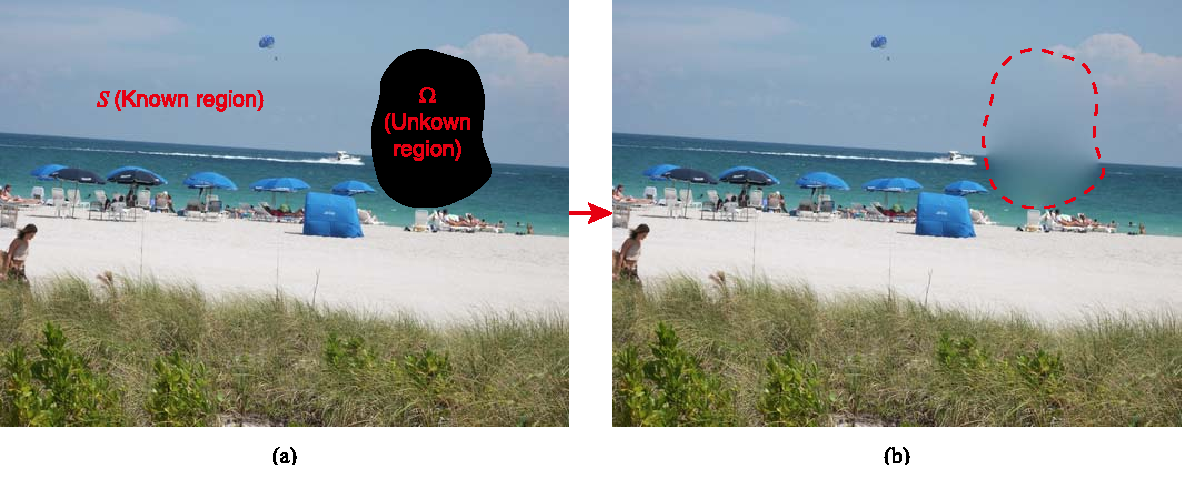
\includegraphics[width=14cm]{figures/diffusion_based_inpainting.png}
    \caption{Diffusion-based inpainting example \cite{diffusion_based_inpainting}}
    \label{fig:diffusion_based_inpainting}
\end{figure}

Another traditional inpainting study based on fast marching method \cite{telea} proposed that, in order to estimate the color of the missing pixels, gradients of the neighbor regions can be used. In our work, these two methods used as a baseline when comparing the deep learning based inpainting methods with traditional inpainting methods.

\subsection{Navier-Stokes Method}

Navier-Strokes equations are partial differential equations for describing the motion of fluid substances. These equations used in variety of areas in different industries such as modeling ocean currents, weather conditions and even when designing aircrafts and cars. However, there is no proof for solutions exist, and are they unique?These revolutionary equations In 2000, the Clay Mathematics Institude made this problem one of the seven millennium prize problems \cite{clay} offering a one million dollar prize to the first person providing a solution.



\subsection{Fast Marching Method}

Enes yazacak.